\documentclass[10pt,twocolumn,letterpaper]{article}

\usepackage{cvpr}
\usepackage{times}
\usepackage{epsfig}
\usepackage{graphicx}
\usepackage{amsmath}
\usepackage{amssymb}
\usepackage{multirow}
\usepackage{lscape}

% Include other packages here, before hyperref.

% If you comment hyperref and then uncomment it, you should delete
% egpaper.aux before re-running latex.  (Or just hit 'q' on the first latex
% run, let it finish, and you should be clear).
\usepackage[breaklinks=true,bookmarks=false]{hyperref}

\cvprfinalcopy % *** Uncomment this line for the final submission

\def\cvprPaperID{****} % *** Enter the CVPR Paper ID here
\def\httilde{\mbox{\tt\raisebox{-.5ex}{\symbol{126}}}}

% Pages are numbered in submission mode, and unnumbered in camera-ready
%\ifcvprfinal\pagestyle{empty}\fi
%\setcounter{page}{4321}
\begin{document}

%%%%%%%%% TITLE
\title{New York State Inpatient Healthcare Data Analysis and Cost Prediction}

\author{Justin Yong Sik Cho\\
Columbia University\\
{\tt\small yc3522@columbia.edu}
% For a paper whose authors are all at the same institution,
% omit the following lines up until the closing ``}''.
% Additional authors and addresses can be added with ``\and'',
% just like the second author.
% To save space, use either the email address or home page, not both
\and
Yuan-Fang Lin\\
Columbia University\\
{\tt\small yl4042@columbia.edu}
\and
Jing Qian\\
Columbia University\\
{\tt\small jq2282@columbia.edu}
}

\maketitle
%\thispagestyle{empty}

%%%%%%%%% ABSTRACT
\begin{abstract}
%Abstract: Briefly describe your problem, approach, and key results.
    Healthcare in the United States is increasingly becoming the center of national attention especially due to its quick growth in spending. In fact, healthcare spending in the US grew 4.6\% in 2018 surpassing \$ 3.6 trillion or \$11,172 per person. With 17.7\% of the country's Gross Domestic Product spent on healthcare, monitoring the vast amount of data on how people incur costs is increasingly becoming an area of interest.
    %https://www.cms.gov/Research-Statistics-Data-and-Systems/Statistics-Trends-and-Reports/NationalHealthExpendData/NationalHealthAccountsHistorical
    Big data analytic technologies in the modern era enables users to sift through the high volume of healthcare records and extract insights that point to systematic patterns or leverage machine learning to build useful applications. Previous research aimed to test for bias in various fields ranging from healthcare practices to police violence. These works provided guidance on which features to explore to test for bias, while shedding light on potential limitations and difficulties such as data-resolution and underlying distributions that can complicate analyses. Our project aims to build on these findings by....[add point on where our work adds values yc3522 yl4042]. Our research aims to close this gap while focusing on a subset population in New York State. We perform experiments to test for systemic bias across sensitive class labels, identify potential patterns and clusters in the inpatient population, and finally develop a prediction tool which helps users estimate the cost of healthcare given general user information. We make our data, models, and code available on Github\footnote{https://github.com/justinchoys/nyhealth-bigdata}. Through statistical analysis, we found that race, gender and age bias exist significantly in the discharge costs per day and the bias vary from county to county.%[add quick summary of experiment findings jq2282]
\end{abstract}

%%%%%%%%% BODY TEXT
\section{Introduction}
% Describe and define the problem you are working on. Why is it important? Include an overview of your methods and results.

Healthcare spending over the past decade has grown at a considerable pace in the United States. Especially in New York state, the annual average rate of growth in per-person spending of health-care from 2013 to 2017 was 6.2\%, compared with 3.9\% nationally. The interest in healthcare has also soon ballooned into the point of popularity. In order to better understand the trends in healthcare, our work focuses on a relatively high-resolution data set based in New York State inpatient discharge records, which offer valuable information such as patient demographics, healthcare geographies, and healthcare cost, all without compromising privacy laws. More specifically we clean the data set, employ statistical tools to select key features, and test for biases among the variables to identify if there are systemic patterns of unequal treatment and costs across different independent groups. We use ANOVA to find significant features that contribute to the mean discharge cost. With ANOVA, we could figure out wether there exist race, gender and age bias in mean discharge costs. Once we find the bias features, we will Tukey method to perform multiple-comparison test and find whether there are significant difference among groups of these bias features. We also aim to develop a tool to help predict healthcare costs given basic demographic and geographic inputs. This tool is designed to help potential patients with limit information about diagnosis and medical information to gain insight into what healthcare costs can potentially amount to. Finally, we package our analyses in a Django web application to enable user interactions, inputs, and visualization of results. %[summarize results jq2282]

% \begin{figure}
% 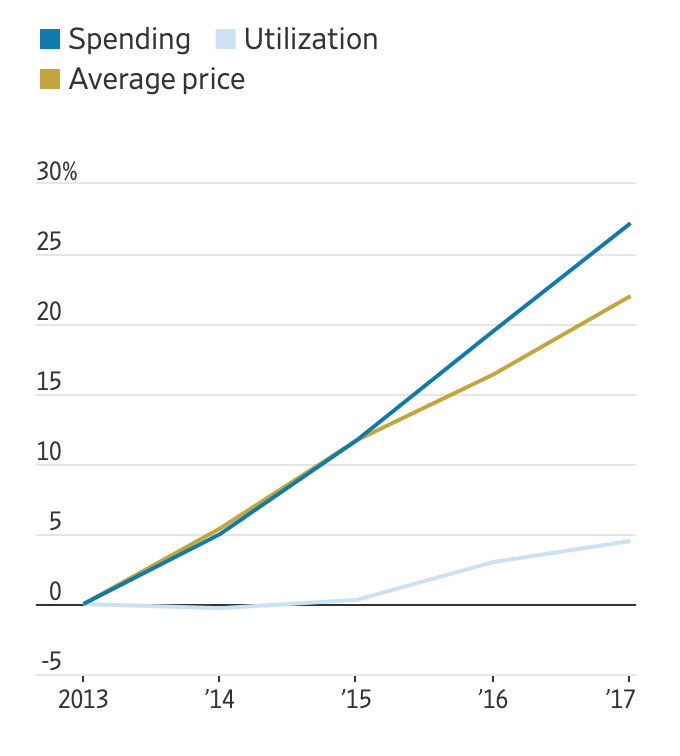
\includegraphics[scale=0.65]{img1.png}
% \caption{Based on values per person. Source: Health Care Cost Institute}
% \end{figure}


\section{Related Works}
% Discuss published works or approaches that are related to your project. What’s the benefit or drawback of the previous works? What kind of problems have they solved? How is your approach similar or different from others?

%1. summarize related works on bias detection, and healthcare data analysis (include URL, abstract, high-level summary of approach used)
%2. merge summaries into entire section

% https://www.ncbi.nlm.nih.gov/pmc/articles/PMC4638275/
Bias is a prejudice against any one of the things in the world, no matter person, or group compared with another usually in a way that is considered to be unfair. Bias may exist toward any social group. One's age, gender, gender identity physical abilities, religion, sexual orientation, weight, and many other characteristics are subject to bias. One particular type of bias is called unconscious bias, also known as implicit bias. Unconscious biases are social stereotypes about certain groups of people that individuals form outside their own conscious awareness. The paper, \textit{Implicit Racial/Ethnic Bias Among Health Care Professionals and Its Influence on Health Care Outcomes: A Systematic Review} \cite{AMJPublicHealth1} provides a useful summary of investigation to which implicit racial/ethnic bias exists among healthcare professionals and examination the relationships between health care professionals’ implicit attitudes about racial/ethnic groups and health care outcomes. The research results provide insights into healthcare practices and suggests that most healthcare providers appear to have implicit bias with positive attitudes towards White patients and negative attitudes toward people of color.

% https://www.ncbi.nlm.nih.gov/pmc/articles/PMC4634878/#pone.0141854.ref039
Another point we focus on in our project is how geography relates to the bias in healthcare costs. \textit{A Multi-Level Bayesian Analysis of Racial Bias in Police Shootings at the County-Level in the United States, 2011–2014} \cite{PLOS1} utilizes a geographically-resolved, multi-level Bayesian model to analyze the extent of racial bias in the shooting of American civilians by police officers in recent years. The research suggests that aside from easily observable bias across Race/Ethnicity or Armed Versus Unarmed by Race/Ethnicity, county-level data are far too coarse to reliably tease apart the conditions that drive racial bias in police shootings. This suggest that although bias may exist in reality, limitations in data and privacy concerns can hinder the ability to find more reliable evidence of such bias.

% (optional) explore works on how to predict cost using healthcare data (categorical)
% https://www.ncbi.nlm.nih.gov/pmc/articles/PMC5977561/
To predict healthcare charges, \textit{Supervised Learning Methods for Predicting Healthcare Costs: Systematic Literature Review and Empirical Evaluation} \cite{AMIA1} implements several learning methods, including Lasso, Ridge, Elastic Net, Random Forest, Support Vector Machine, Gradient Boosting and Artificial Neural Network to review the literature of healthcare cost prediction. One observation that is highlighted is that [yl4042 what is cost on cost? >>>] cost on cost prediction performs as well or even better than predictions using clinical data or clinical and cost data. The researchers also point out that the prediction performance based on statistical model is further complicated by the skewed nature of healthcare data, where distributions are strongly skewed with different bias and extreme values can be present, all of which make it inefficient to use small to medium sample sizes if the underlying distribution is not normal. As a result, we chose to first focus on investigating the distribution of data and the multiple bias that exist in the data set before proceeding to implement a prediction model for potential healthcare-charge using high-level user information.

% A Preprocessing Scheme for High-Cardinality Categorical Attributes in Classification and Prediction Problems. 
% http://helios.mm.di.uoa.gr/~rouvas/ssi/sigkdd/sigkdd.vol3.1/barreca.pdf

% bridge
The rest of this report is structured as follows: In Section 3, we describe the data with its features and the preprocessing techniques used to reduce the size of data, and in Section 4, we present the principal methods used to analyze and test for bias in our data set as well as the approach and rationale behind our prediction model. In Section 5, we report on the bias results we found among the data set and several simple comparison of performance of our prediction models. Lastly, Section 6 and 7 covers the software architecture and tech stacks of our application and discuss some potential future works and bottlenecks.

\section{Data}
% Describe the data you are working with for your project. What type of data is it? Where did it come from? How much data are you working with? Did you have to do any preprocessing, filtering, feature engineering, or other special treatment to use this data in your project

The data used was sourced from the New York State Hospital Inpatient Discharges (SPARCS De-Identified): 2017\footnote{https://on.ny.gov/2qa8Qlm} data set which contains detailed patient discharge characteristics, diagnoses, treatments, services, and charges. While the record-level data points represent individual patient discharge instances, the data is already de-identified and so does not contain protected  health information under HIPAA. The records are not individually identifiable as well through redaction or aggregation at a lower-resolution scale (e.g. age is categorized into groups rather than specific numbers). Overall, there are 2,343,569 records in the 2017 data set, with each row made up of 34 features including age, gender, zip code, ethnicity, race, and diagnosis. 

%[include table of features (categorized by type of information... e.g. patient information, payment, medical, etc ] 

\subsection{Data Preprocessing}
To ensure consistency of units across all data records, the first step in data preprocessing was normalizing the healthcare costs by the length of stay for each record. This was driven by the motivation to ensure meaningful comparisons across individual entries and also to ensure that all samples were not missing these features. The next step was dropping rows with missing values in certain columns. While most of the records were not missing values (excluding payment types which had anywhere from one to three payment types per record), we specifically elected to drop records that were missing `Hospital Service Area', `Zip Code - 3 digits', and the `APR Risk of Mortality' fields because the records with missing data of these three columns are no more than 2\% of the total data set while the missing input of payments take around 40\% of the total.

We also removed columns containing irrelevant and collinear/repeated information. The columns we dropped include `Discharge Year', `Abortion Edit Indicator', `Operating Certificate Number', `Permanent Facility Id', `CCS Diagnosis Code', `CCS Procedure Code', `APR MDC Code', `APR Severity of Illness Code' and`APR DRG Code'. We specifically elected to remove the abortion edit indicator because there are no abortion records if we remove the rows with NA values and payment types. The remaining dropped columns were removed due to collinearaity. For example, columns beginning with `CCS Diagonosis' contained one-to-one correspondences between codes and descriptions. In order to simplify the data set we dropped the codes while keeping the descriptions because the latter is more human-readable.

\subsection{Data Exploration}
%TBD: distribution et al. 

%How is the sample distributed across Age Groups? Does cost vary with Age or Gender within each Age Group??

%Does average healthcare cost vary across Genders? Are Genders evenly distributed in the sample?


%How is the sample distributed across Race? Do certain races have higher average costs? What about Genders within Race?

%How are features and healthcare costs distributed? (e.g. Age, Gender, Race, Diagnosis)


\subsection{Feature Selection}
The third step is feature selection driven by data exploration and analyses. Once the data was pared down to 20 columns, there were some interesting patterns in the data. Some columns were numerical, like length of stay while some columns were categorical with cardinality in the hundreds, which hinders the modeling process. To tackle this issue, we factorized all the categorical variables  and computed the Pearson correlation matrix among all the variables to inform the feature selection process in Table \ref{CM1} and Table \ref{CM2}.

The correlation between length of stay and total charges was relatively high around 0.7, which motivated our decision to normalize healthcare costs by the length of stay and use this as the dependent variable. 
Other than gender, race and age, location of the hospitals also proved to play an important role in predicting costs. We found moderate correlation between and among geographical variables and facilities related variables. Among all these variables, `Hospital County' had a moderate number of categories and its count distribution was relatively even, which convinced us to use this variable as a representative feature that captured all relevant geographic information.
We also expected the diagnosis features to be useful in predicting healthcare costs given. This is because complex diagnoses and procedures are typically associated with higher costs (e.g. various types of cancer) as opposed to simpler diagnoses and procedures such as the common cold. The data set had four medical diagnosis-related variables with each over 200 categories, which made it difficult to model. However, after we found that there was moderate correlation among these variables, we choose `CCS Diagnosis Description' to represent all medical diagnosis-related information given that this feature was easy to understand and also because it was easy to filter. We also noticed that some diagnoses categories had low frequencies (i.e. rare or infrequent diagnosis) while only a few diagnoses had relatively high frequencies. Because of the disparity in data availability among diagnosis, we decided to limit our bias analysis to the top diagnoses categories.

%TBD: correlation matrix

%=======================================================================%

\section{Methods}
%Discuss your approach for solving the problems that you set up in the introduction. Why is your approach the right thing to do? Did you consider alternative approaches? Have your tried some methods that didn’t work out? It may be helpful to include figures, diagrams, or tables to describe your method or compare it with other methods.

% [TALK ABOUT BIAS METHODOLOGY]
For the bias analysis, we used a widely used method in statistics, ANOVA. ANOVA refers to analysis of variance, which is based on the law of total variance, where the observed variance in dependent variable is partitioned into componenets attributes to different sources of variation. Specifically, how much of the variance in dependent variable could be explained by the variance between groups in a certain feature and how much could be explained by the variance within groups. 


There are several test methods in the family of ANOVA, like MANOVA for multiple dependent variables, ANCOVA for covariance analysis among continuous independent variables. In our case, considering the independent variables are mainly categorical and there is only one dependent variable, we use ANOVA. 

In ANOVA, a regression model is used to fit the relationship between independent variables and dependent variable. We used R to do the ANOVA bias analysis. We used a linear regression model to fit the mean discharge costs per day and take ten features from previous data preprocessing as independent variables. 

For example, controlling the effects from other variable, if different races have the same effect on the mean charges, then race is not a significant feature and there is no racial bias in mean charges. 

used to identify which features in a model are significant. 

The basic idea is to check how observed variances in the response variable is explained by a specific model instead of random samples. %[jq2282 i don't understand what you mean by 'while other variables are similar'] %From our ANOVA analysis, we could see that all these ten features are significant in explaining the mean charges for “Liveborn”.

Once we identified what types of biases exist in features (e.g. gender, race, and age) , we explored how the mean charges differ among different groups of the features and tested these differences for statistical significance. To compute this, we required a multiple-comparison test. Here, we used Tukey’s HSD (honestly significant difference) method, which is a single-step multiple comparison procedure and statistical test. The basic idea of Tukey’s method is compute pairwise comparisons between different groups in the variable. It is essentially a t-test, except that it corrects for family-wise error rate.

%% ^^^ Our main part in Methods and Experiments will the bias one. More elaboration is better  jq2282 :)

% [TALK ABOUT CLUSTERING/TSNE WHICH DIDN'T WORK OUT]
After choosing to focus on the five categorical features, we first decided to analyze the data through clustering. We randomly picked 100,000 sample points and implemented the K-means algorithm and also the tSNE method for visualization. As expected, in Figure 1 and Figure 2, due to these extremely sparse features and presence of many outliers with extreme values, the within-set-sum-of-squared-error is unacceptably large. We could not claim that there is a stable or meaningful clustering of the sample data, even after using the 3D-tSNE method preceded by a Principal Component Analysis (PCA) step. However, when clustering on a smaller sample size, we can still visually observe clustering as shown in red, light green and dark blue regions in Figure 3.

% [TALK ABOUT PREDICTION MODEL]
Another component of our project involved building a prediction model to estimate healthcare costs per day using only high-level user information. This application is designed to be useful in real-world scenarios such as for potential patients who wish to estimate healthcare costs prior to a hospital visit and diagnosis. Leveraging our results from bias detection, we elected to include race, gender and age group information as key input variables that can reliably predict healthcare costs. Taking into account applicability to real-world scenarios that often come with limited information, we decided to add two more features as inputs: `Zip Code' and `Type of Admission'. Due to the categorical data type that dominated our features as opposed to the numeric label (healthcare cost per day), we determined that a decision tree model was the best candidate model type to use due to its ability to handle large amounts of categorical inputs. We utilized one-hot encoding to vectorize our categorical input features (`Race', `Gender', `Age Group', `Zip Code', and `Type of Admission') which resulted in an extremely sparse feature vector. The sparse feature vector implied that a neural network model for the prediction task would be difficult unless the network had sufficient depth and additional network features such as penalizing results if insufficient neurons fired in the training phase. To avoid this pitfall, we instead relied on using gradient boosting techniques, which produces a prediction model with an ensemble of weak prediction models, which typically comprise of decision trees. 
As an experiment, we tested another approach for the prediction task using a simple artificial neural network despite our initial concerns, which surprisingly yielded moderately better results with almost a 50\% reduction in RMSE over the Gradient Boosted Regressor model on the same sample data set. Table 1 shows the resulting RMSE differences between the Gradient Boosted Regressor and two neural networks with different number of layers. We used stochastic gradient descent as the optimizer with a learning rate of 0.1. The neural networks were configured to be a fully-connected network with each layer followed by relu activation functions. The 3-Layer neural network has two hidden layers which respectively has 32 and 8 neurons and the 5-layer neural network has four hidden layers which in each has 32, 16, 8, and 4 neurons.

\begin{figure}
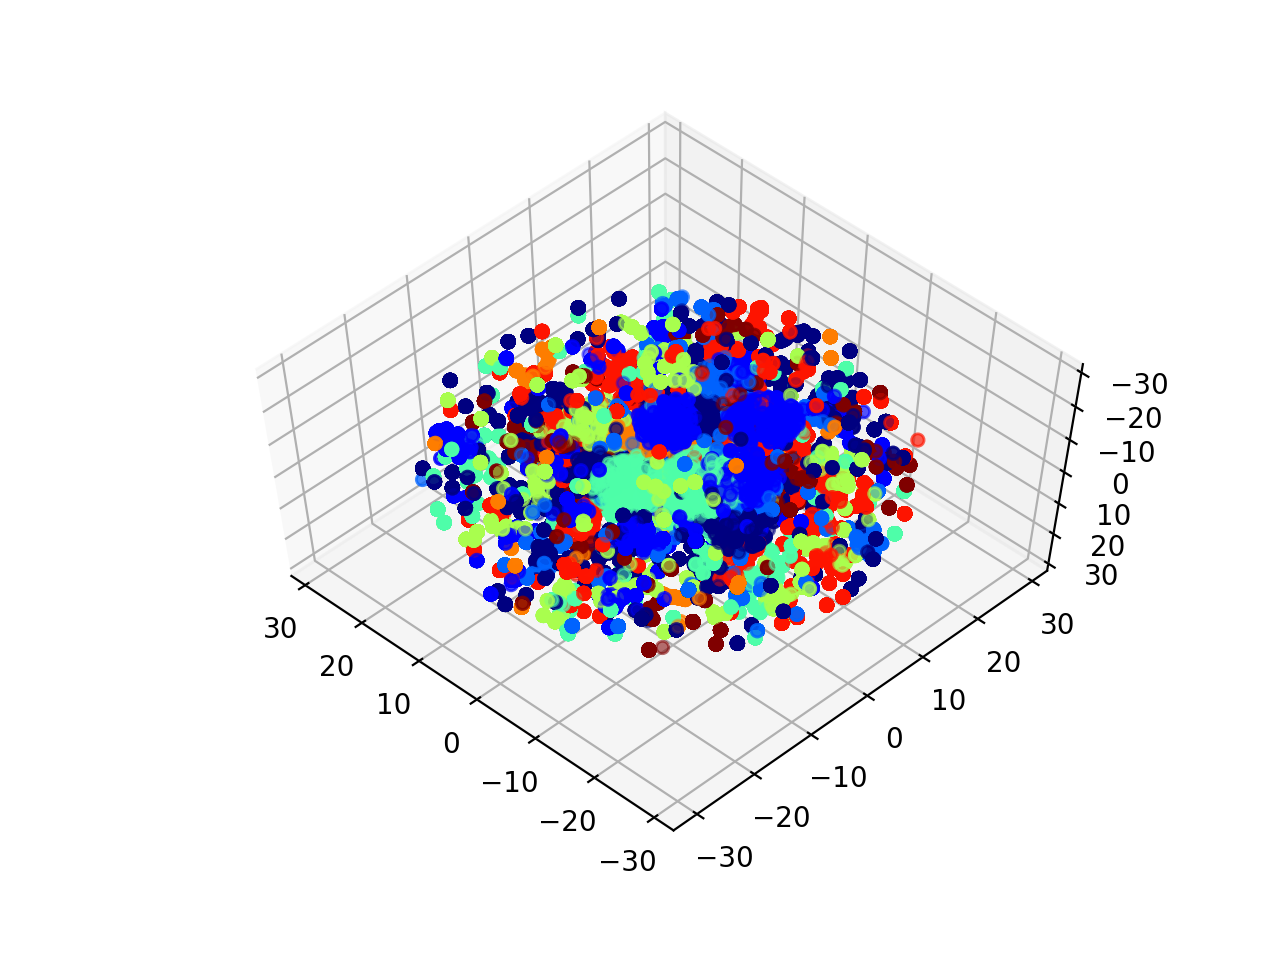
\includegraphics[scale=0.5]{100k-tsne.png}
\caption{100K Data visualization with PCA and 3D-tSNE}
\end{figure}

\begin{figure}
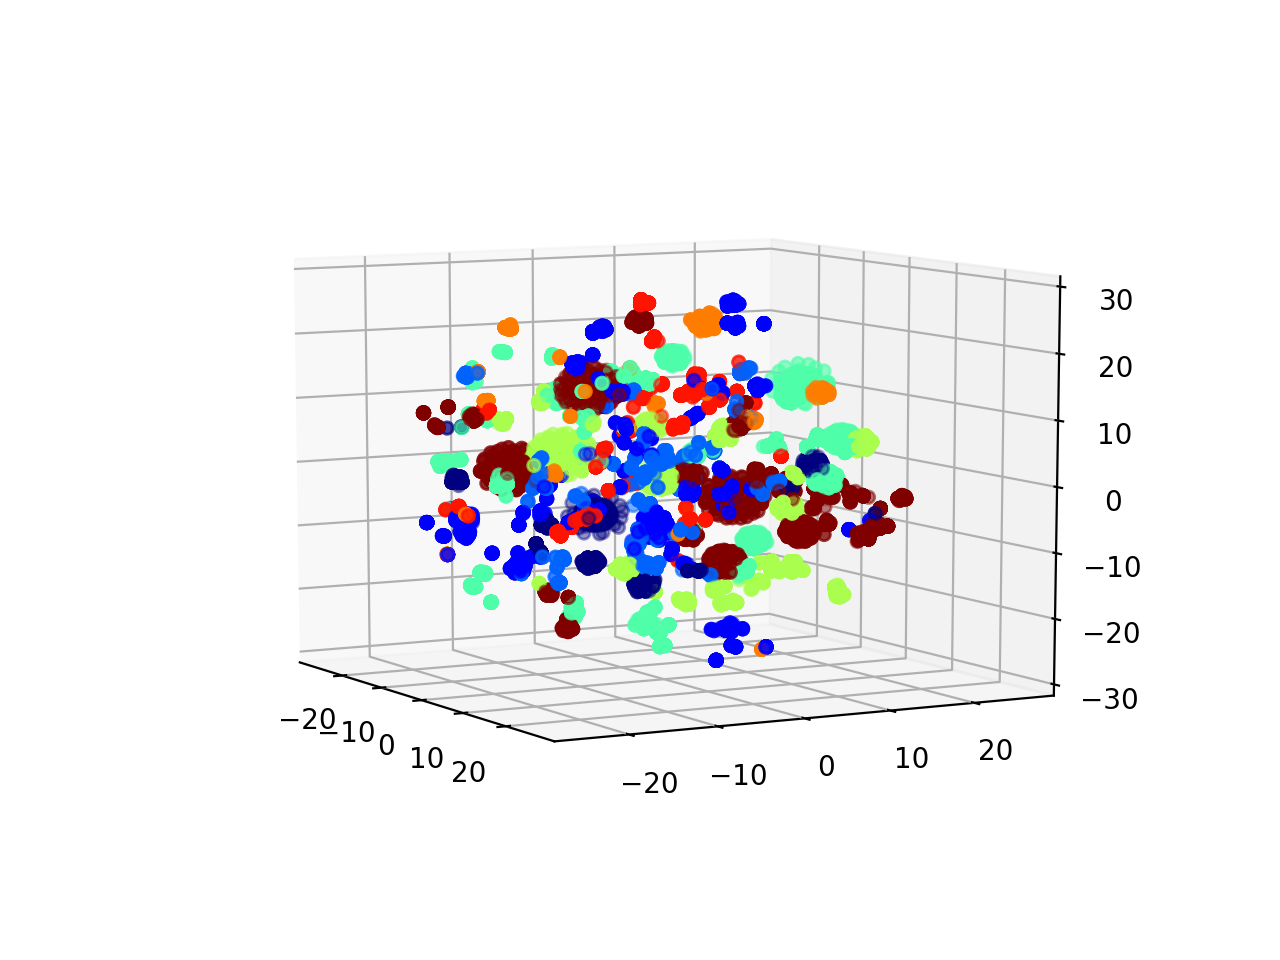
\includegraphics[scale=0.5]{10k-tsne.png}
\caption{10K Data visualization with PCA and 3D-tSNE}
\end{figure}

\begin{figure}
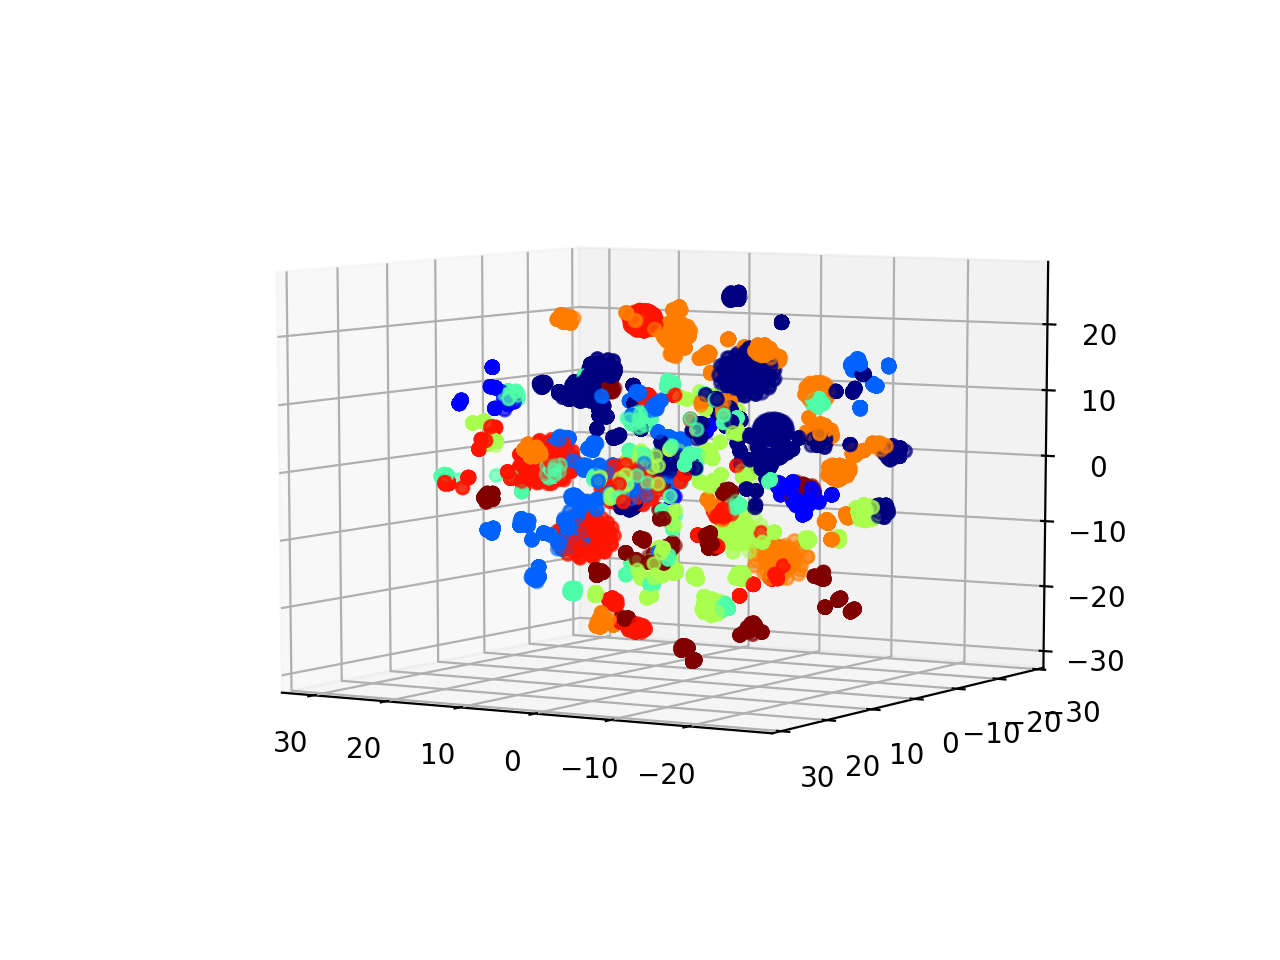
\includegraphics[scale=0.5]{1k-tsne.png}
\caption{1K Data visualization with PCA and 3D-tSNE}
\end{figure}

%=======================================================================%

\section{Experiments}
%Discuss the experiments that you performed to demonstrate your approach solves the problem. The experiments will vary depending on the project, but you might compare with previously methods, determine the impact of the components of your system, experiment with different hyper-parameters, architectures, or algorithms, use visualization techniques to gain insight of how your model works, etc. Graphs, tables, and figures are highly recommended to be included to illustrate your experimental results.

% [Talk about bias detection here as experiment... how did we experiment with variables to identify "across which feature does healthcare cost bias exist?"]
After feature selection, we successfully reduced our feature numbers to 10 [jq2282 which 10 features? can you include table please]. Here we took the top diagnosis category - `Liveborn' (over 9\% of the whole data) as an example to demonstrate the bias analysis. It is worth noticing that the patients of `Liveborn' are newborns, not the mothers. There is only one age category: between 0 and 17 and hence no possible age bias. However, there is a possibility that there are gender biases among the newborns. To test for this, we used ANOVA to test for which features of records were significant in explaining the variance in healthcare costs. From our ANOVA analysis, we could see that all these ten features were significant in explaining the mean charges for `Liveborn'.

% [TALK ABOUT SOME EXP ABOUT NN]
We have included in Table 1 a summary of the performance between the two approaches to implementing a healthcare cost prediction model. The results indicate that in contrast to our expectations, neural networks yielded better performance as shown by the significantly lower RMSE value. All models used in the experiment are trained on the same subset of 1 million records randomly sampled from the SPARCS 2017 data set. As we can see, neural network depth does not appear to have much impact on prediction performance. This may be driven by the sparsity of the vectorized features. Without a truly deep neural network it does not seem likely that incremental increases in network depth will result in significant performance improvements. We also conducted experiments to test the performance of the neural networks using different hyper-parameters, including learning rate and type of optimizer. Table 2 summarizes the results from varying the learning rate hyper-parameter and suggest that learning rate can significantly affect the supervised learning process and resulting performance. Similarly, Table 3 shows the the result from varying the optimizer, indicating that the Adam optimizer yielded the best performance for the 3-layer network. Finally in Table 4, we show the impact of varying maximum tree depth and iteration on the Gradient Boosted Regressor model. For all models, the selected features were vectorized into 63 ($\approx 2^6$) dimensional records, which explains how the model with maximum depth 10 tended to perform better.


\begin{table}[t!]
\small
\begin{center}
\begin{tabular}{|c|c|c|c|}
\hline
     & \textbf{GBTRegressor} & \textbf{NN(3-Layer)} & \textbf{NN(5-Layer)}\\ \hline
\textbf{RMSE} & 12401.1     & \textbf{6939.7012}  &  6940.5825                     \\ \hline
\end{tabular}
\end{center}
\caption{ RMSE of GBTRegressor (maxDepth=10, maxIter=30), 3-Layer Neural Network and 5-Layer Neural Network. All trained on 1M data sample with 80/20 train-test split}
\end{table}

\begin{table}[t!]
\small
\begin{center}
\begin{tabular}{|c|c|c|c|}
\hline
     & \textbf{NN(3-Layer)} & \textbf{NN(5-Layer)} \\ \hline
\textbf{lr = 0.1} & 6939.7012 & 6940.5825     \\ \hline
\textbf{lr = 0.05} & 6939.1870 & 6939.2915     \\ \hline
\textbf{lr = 0.001} & \textbf{5785.8926} & 10235.0606     \\ \hline
\end{tabular}
\end{center}
\caption{RMSE of neural network models with 60 epochs, 32 as batch\_size and SGD as optimizer with varying learning rates}
\end{table}

\begin{table}[t!]
\small
\begin{center}
\begin{tabular}{|c|c|c|c|}
\hline
     & \textbf{NN(3-Layer)} & \textbf{NN(5-Layer)} \\ \hline
\textbf{SGD} & 5785.8926 & 10235.0606 \\ \hline
\textbf{Adam} & \textbf{5705.9321} & 9835.3730 \\ \hline
\textbf{AdaGrad} & 6492.8960 & 6149.6025 \\ \hline
\end{tabular}
\end{center}
\caption{RMSE of neural network models with 60 epochs, 32 as batch\_size and 0.001 as learning rate with varying optimzers}
\end{table}

\begin{table*}[t!]
\small
\begin{center}
\begin{tabular}{|c|c|c|c|}
\hline  \textbf{Training Data Size} & \textbf{Maximum Depth} & \textbf{Maximum Iteration} & \textbf{RMSE}  \\ \hline
\multirow{4}{*}{10K}  & 10 & 30 & 9679.85  \\ 
  & 10 & 50 & \textbf{8890.98}  \\
  & 20 & 50 & 10207.5  \\
  & 20 & 30 & 10091.7  \\ \hline
\multirow{4}{*}{100K}  & 10 & 30 & 12049.1  \\ 
  & 10 & 50 & 12574.1  \\
  & 20 & 50 & \textbf{11889.6}  \\
  & 20 & 30 & 12182.7  \\ \hline
%\multirow{4}{*}{500K}  & 10 & 30 & 11829.7  \\\
%  & 10 & 50 & 11927.8  \\
%  & 20 & 50 & \textbf{11731.7}  \\
%  & 20 & 30 & 11824.1  \\ \hline
\multirow{4}{*}{1M}  & 10 & 30 & 12688.1 \\
  & 10 & 50 & \textbf{12167.1}  \\
  & 20 & 50 & 12609.1  \\
  & 20 & 30 & 12293.9  \\ \hline
\end{tabular}
\end{center}
\caption{RMSE for different hyperparameters of Gradient Boosted Regressor}
\label{pairwise-summary-table}
\end{table*}

%=======================================================================%

\section{System Overview}
%Describe the software architecture and tech stacks of your application. Discuss potential bottlenecks and improvements that could be made. Mention the software packages that you used. Mention how to use your application. You could provide screenshots to your application.
As shown in Figure 5, we created a front-end website which enables users to visualize various results based on fields and features of their choosing. There are a total of three tabs Home, Dashboard, Prediction and Heatmap, the latter three which focus on the findings and results of our project. Figure 6. illustrates the Home tab which includes a simple introduction to our website application and the data set. For the remaining three tabs, the web application retrieves the information collected from the user and submit a SQL or PySpark Job to BigQuery or Google Cloud Platform Cluster respectively. The Prediction tab, which uses the prediction model, is mainly driven by a model we trained using the SPARC 2017 dataset. Once the user submits the relevant information, .......... [need to rephrase what you are trying to say here yf4042] benefited from PySpark Machine Learning model for Gradient Boosting Regressor and PyTorch for neural network. Figure 7 shows how the Dashboard tab provides users an overview to the data across different user-selected fields. The pie chart and bar chart update in real time based on cursor location over bars/pies and therefore provide an interactive experiencing in analyzing the data. Figure 8 covers the Prediction tab which enables users to input their own information to get two values. The first value returned by the web application is the simple average healthcare cost per day queried from the data set. The second value returned is the predicted result according to our model, which can handle instances and inputs where the SPARC 2017 data set have no historical records to refer to. Finally, Figure 9 demonstrates the Heatmap tab which is a user-friendly visualization of New York state by counties, colored by the differences in average charges per day across user-selected fields such as race, gender, or age groups for a particular diagnosis.
One of the potential bottlenecks to our application is scalability. The current design is able to retrieve the model predicted healthcare cost by submitting a job to a cluster on Google Cloud Platform. This presents a potential scalability issue where multiple users may submit multiple jobs and thus cause significant delays in cluster computing as the cluster is not elastic. In order to alleviate this problem, a potential solution may be to scaling out the clusters and leveraging a load-balancer to separate and direct jobs to idle or available cluster instances.

\begin{figure*}
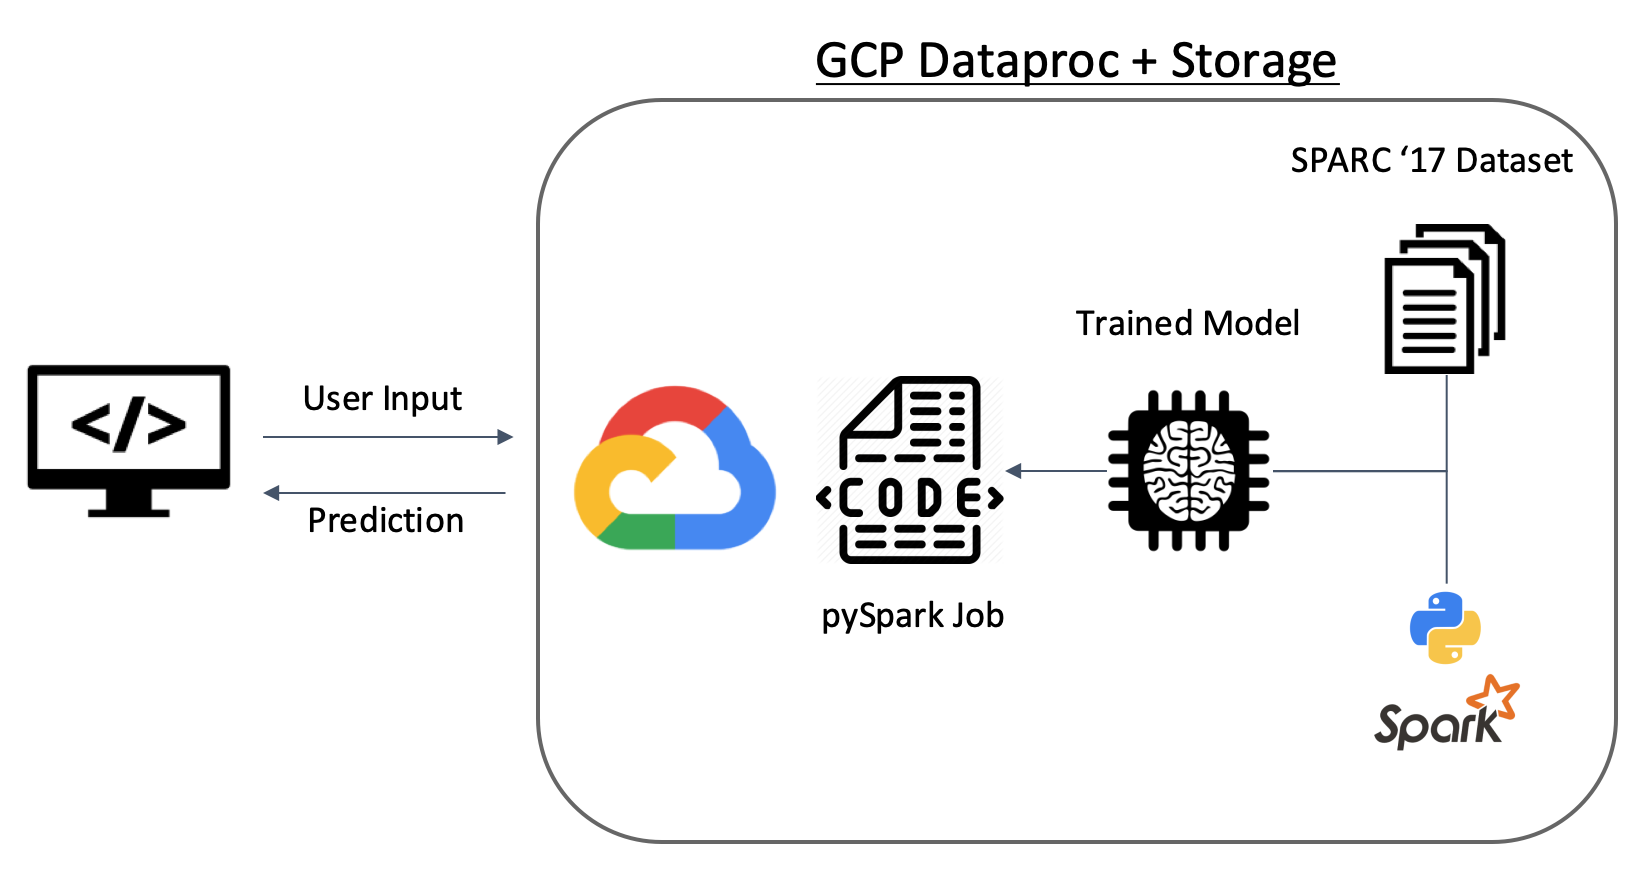
\includegraphics[scale=0.57]{arch.png}
\caption{Application/Software Architecture}
\end{figure*}

\begin{figure*}
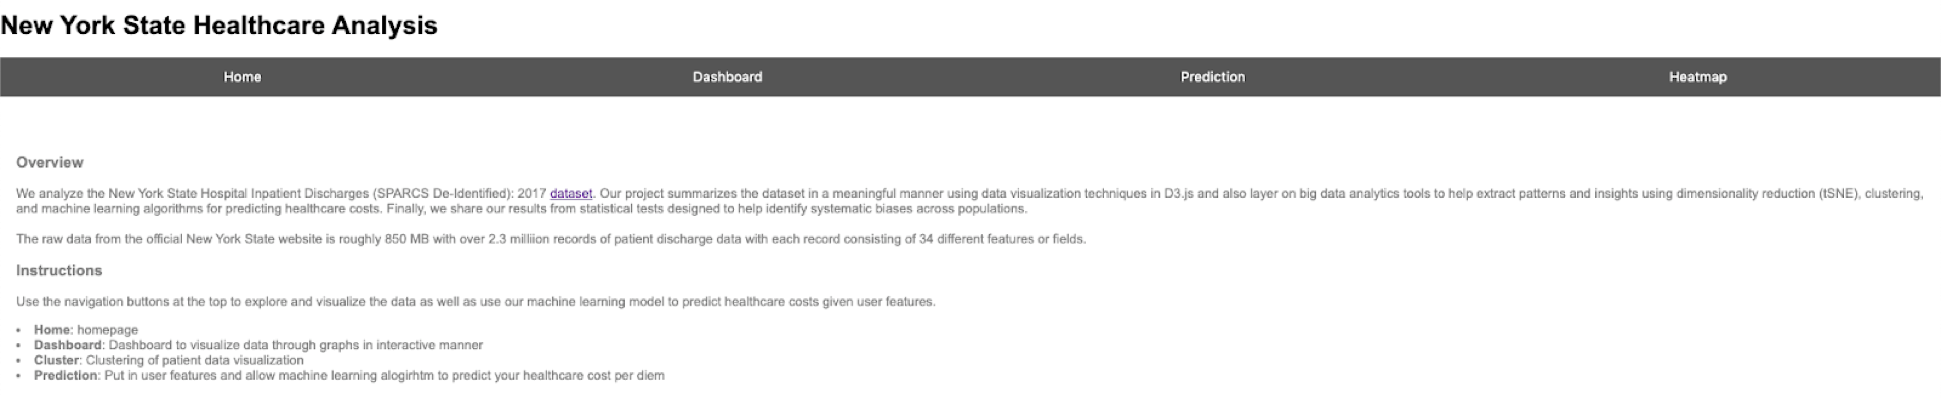
\includegraphics[scale=0.57]{homepage.png}
\caption{Homepage}
\end{figure*}

\begin{figure*}
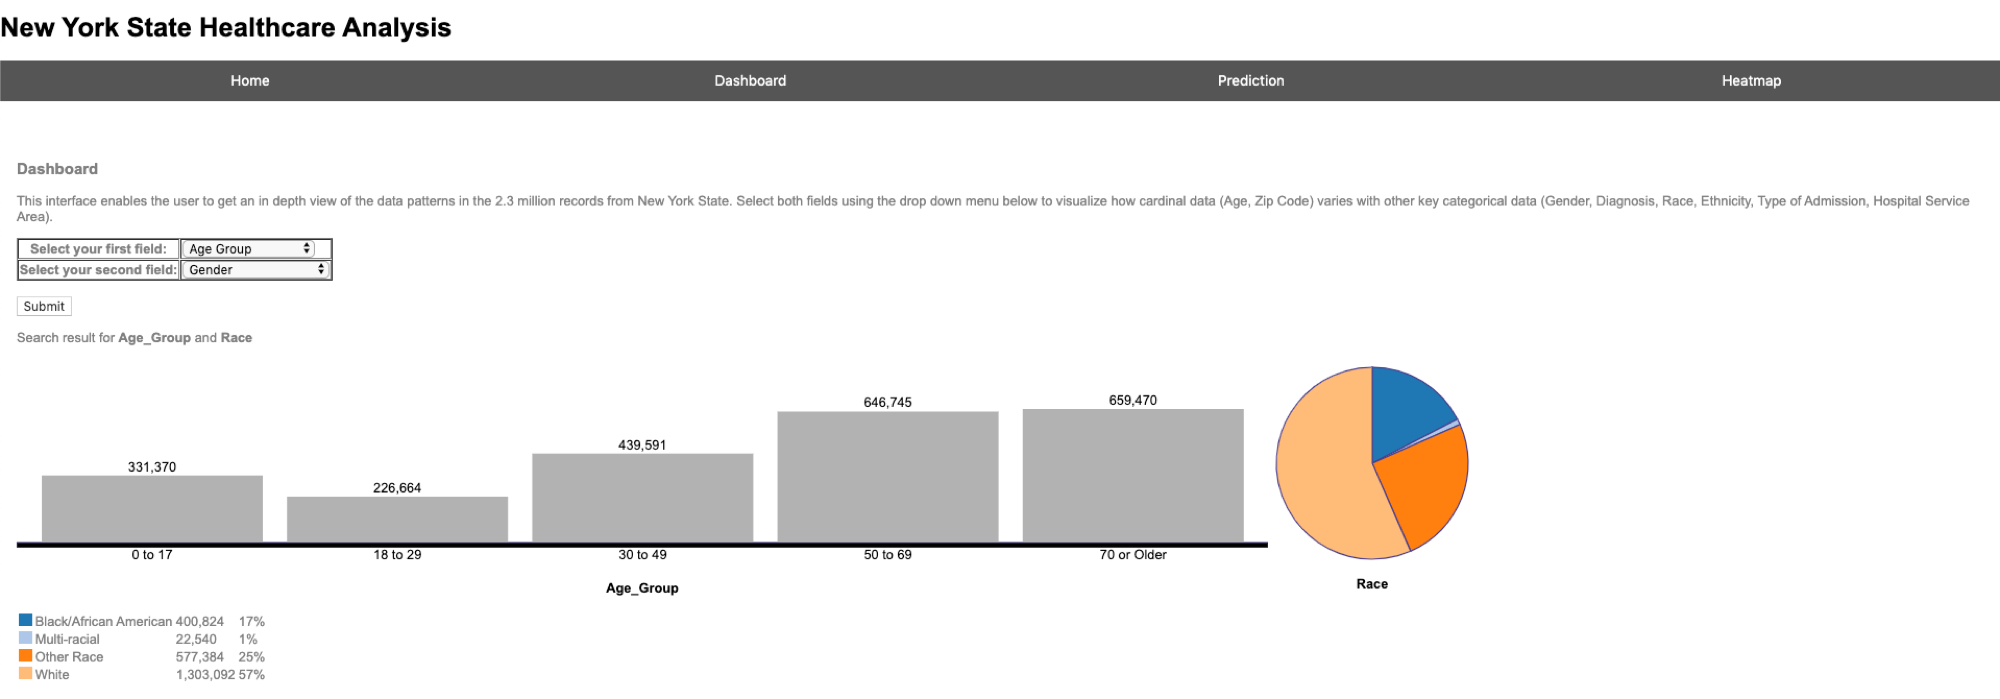
\includegraphics[scale=0.57]{dashboard.png}
\caption{Dashboard tab for data overview}
\end{figure*}

\begin{figure*}
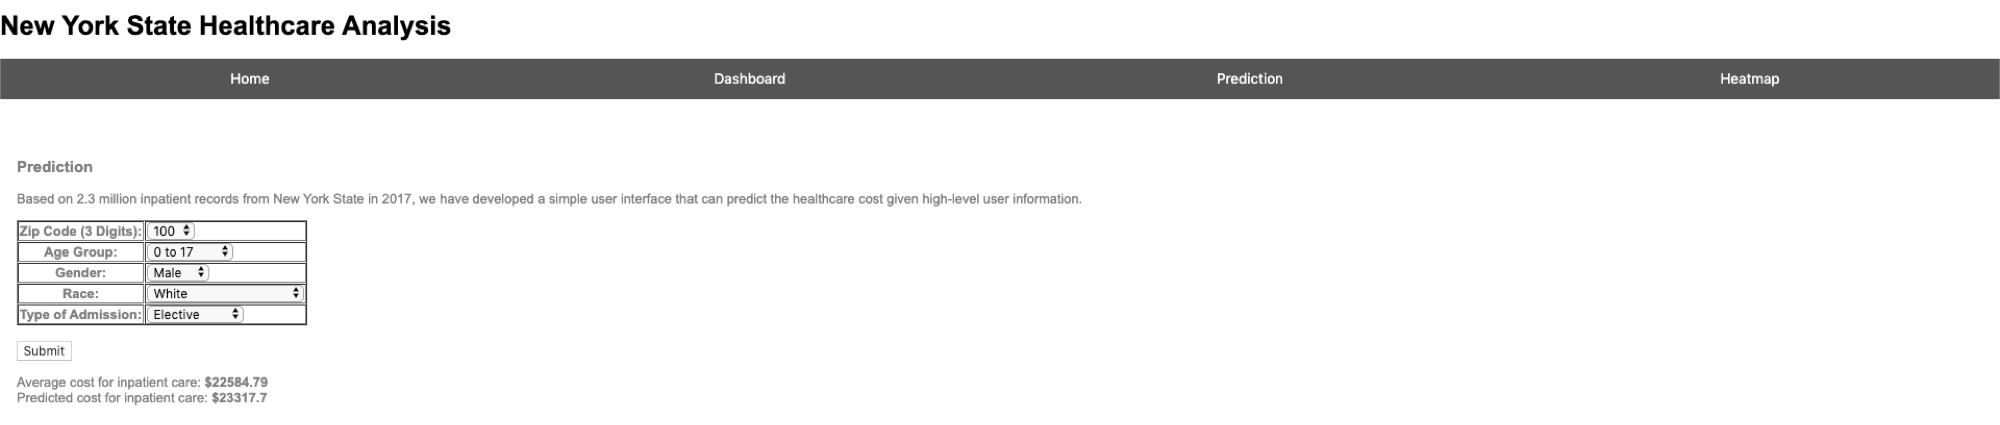
\includegraphics[scale=0.57]{prediction.png}
\caption{Prediction tab for potential healthcare charge according to high-level user information with our model}
\end{figure*}

\begin{figure*}
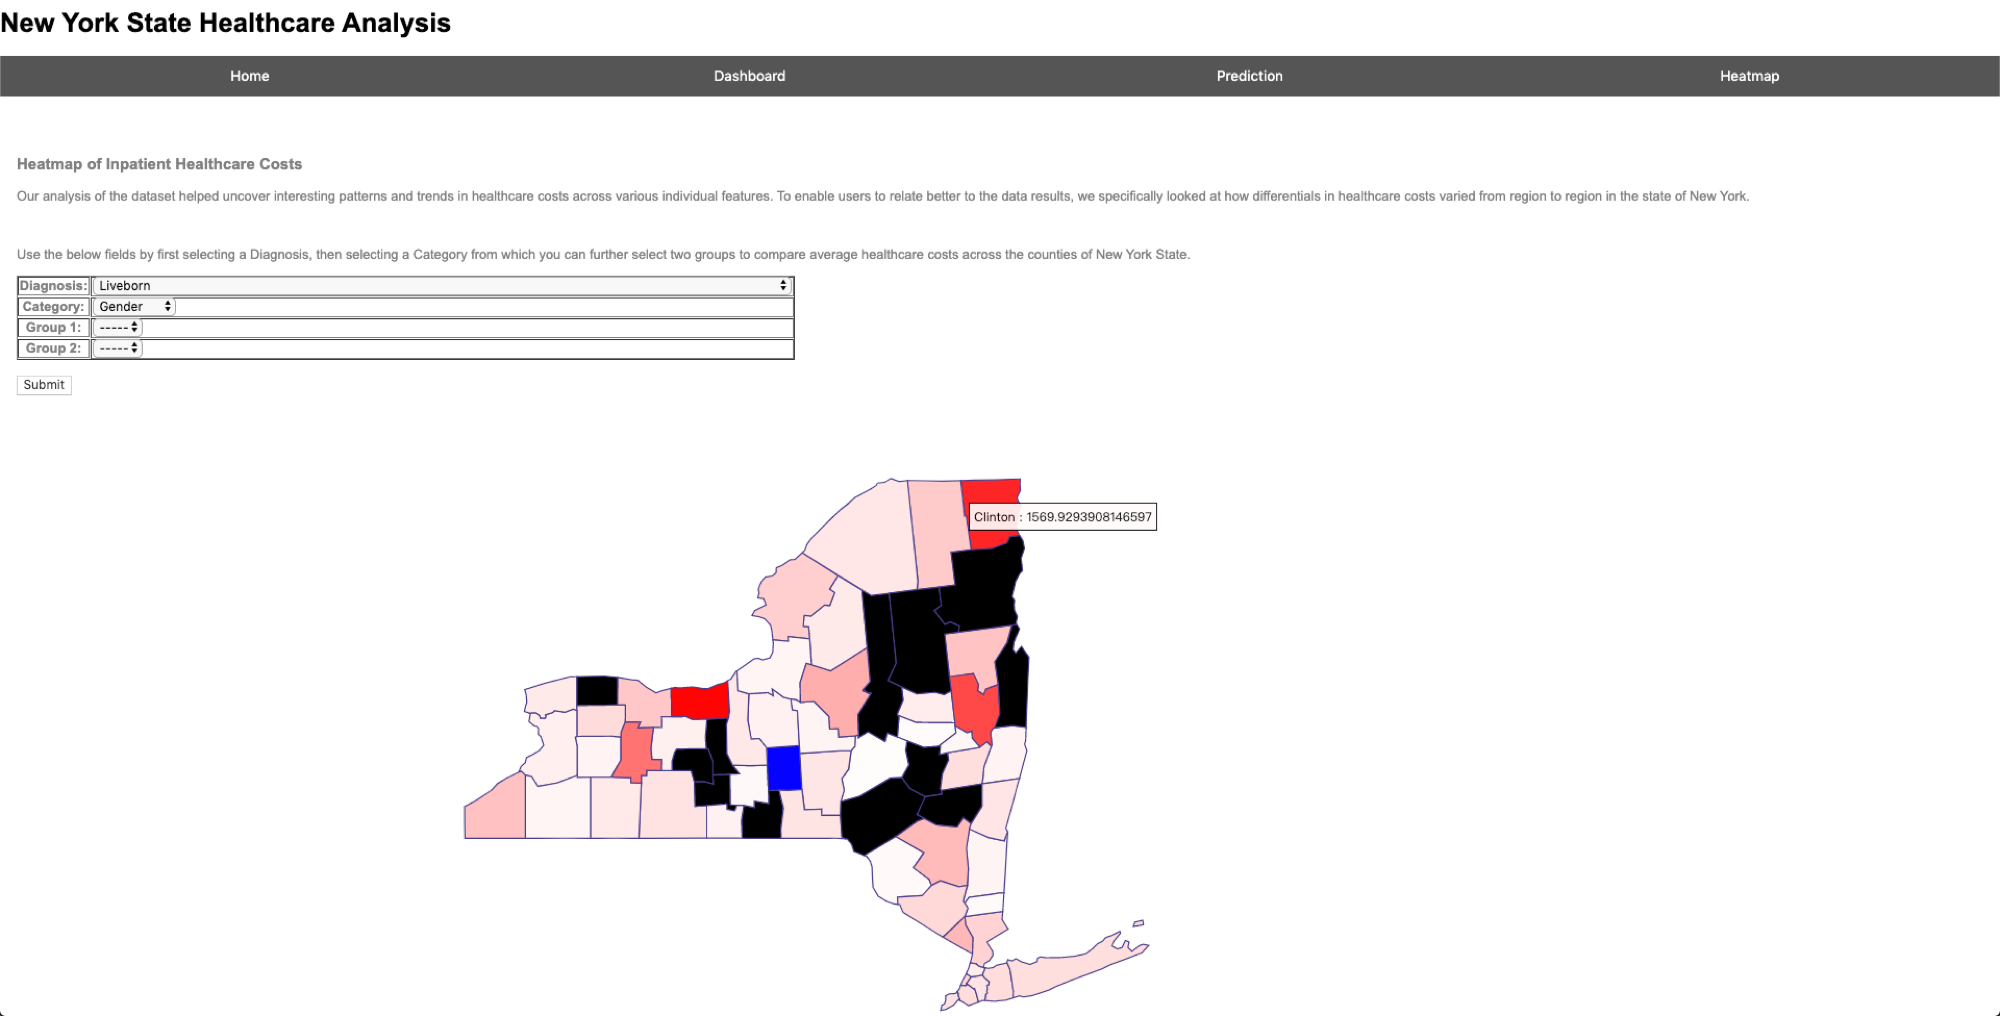
\includegraphics[scale=0.57]{heatmap.png}
\caption{Heatmap tab for user-friendly visualization}
\end{figure*}
%=======================================================================%

\section{Conclusion}
%Summarize your key results. What have you learned? What problems have you discovered and solved? Suggest ideas for future extensions or new applications.

[jq2282 add results]
%=======================================================================%

%Writing / Formatting (4%) Is your paper clearly written and nicely formatted?
%Supplementary Material, not counted toward your 10 page limit. You may include some supplementary materials including but not limited to:
%Code structure.
%Link to your Github repo and youtube video.
%Link to your application if deployed online.

%=======================================================================%


\section{Appendix}
1. Correlation Matrix
% Please add the following required packages to your document preamble:
% \usepackage{lscape}
% Please add the following required packages to your document preamble:
% \usepackage{lscape}
\begin{landscape}
\begin{table}[]
\begin{tabular}{|c|c|c|c|c|c|c|c|c|c|c|}
\hline
                                       & \textbf{Area} & \textbf{County} & \textbf{Facility} & \textbf{Age} & \textbf{Gender} & \textbf{Race} & \textbf{Ethnicity} & \textbf{Admission} & \textbf{Disposition} & \textbf{Diagnosis} \\ \hline
\textbf{Area}         & 1.0000                         & 0.4459                           & 0.2133                             & 0.0107                        & 0.0065                           & -0.2907                        & -0.1767                             & 0.0034                              & 0.0106                                & 0.0099                              \\ \hline
\textbf{County}       & 0.4459                         & 1.0000                           & 0.4288                             & 0.0161                        & 0.0043                           & -0.2904                        & -0.1389                             & 0.0207                              & 0.0018                                & -0.0184                             \\ \hline
\textbf{Facility}     & 0.2133                         & 0.4288                           & 1.0000                             & 0.0189                        & -0.0072                          & -0.1464                        & -0.0932                             & -0.0155                             & -0.0132                               & 0.0082                              \\ \hline
\textbf{Age}          & 0.0107                         & 0.0161                           & 0.0189                             & 1.0000                        & -0.0338                          & -0.0179                        & 0.0322                              & 0.2041                              & 0.0098                                & -0.0683                             \\ \hline
\textbf{Gender}       & 0.0065                         & 0.0043                           & -0.0072                            & -0.0338                       & 1.0000                           & 0.0091                         & 0.0014                              & -0.0249                             & -0.0397                               & 0.0062                              \\ \hline
\textbf{Race}         & -0.2907                        & -0.2904                          & -0.1464                            & -0.0179                       & 0.0091                           & 1.0000                         & 0.3662                              & 0.0355                              & -0.0506                               & -0.0196                             \\ \hline
\textbf{Ethnicity}    & -0.1767                        & -0.1389                          & -0.0932                            & 0.0322                        & 0.0014                           & 0.3662                         & 1.0000                              & 0.0651                              & -0.0397                               & -0.0273                             \\ \hline
\textbf{Admission}    & 0.0034                         & 0.0207                           & -0.0155                            & 0.2041                        & -0.0249                          & 0.0355                         & 0.0651                              & 1.0000                              & -0.0639                               & -0.1522                             \\ \hline
\textbf{Disposition}  & 0.0106                         & 0.0018                           & -0.0132                            & 0.0098                        & -0.0397                          & -0.0506                        & -0.0397                             & -0.0639                             & 1.0000                                & 0.0319                              \\ \hline
\textbf{Diagnosis}    & 0.0099                         & -0.0184                          & 0.0082                             & -0.0683                       & 0.0062                           & -0.0196                        & -0.0273                             & -0.1522                             & 0.0319                                & 1.0000                              \\ \hline
\textbf{Procedure}    & -0.0156                        & -0.0592                          & -0.0301                            & -0.0027                       & -0.0419                          & 0.0075                         & 0.0095                              & -0.0767                             & 0.0030                                & 0.1865                              \\ \hline
\textbf{APR DRG}      & 0.0168                         & -0.0280                          & 0.0072                             & -0.0912                       & -0.0843                          & -0.0245                        & -0.0299                             & -0.1211                             & 0.0581                                & 0.5188                              \\ \hline
\textbf{APR MDC}      & -0.0204                        & -0.0270                          & -0.0181                            & 0.0508                        & 0.0324                           & 0.0288                         & 0.0417                              & 0.0311                              & -0.0365                               & 0.2529                              \\ \hline
\textbf{Severity}     & -0.0086                        & -0.0065                          & -0.0023                            & 0.0882                        & 0.0069                           & 0.0223                         & 0.0235                              & 0.0660                              & -0.0160                               & -0.0326                             \\ \hline
\textbf{Mortality}    & 0.0469                         & 0.0427                           & 0.0007                             & 0.1297                        & -0.0804                          & -0.0949                        & -0.0756                             & -0.0223                             & 0.2841                                & -0.0332                             \\ \hline
\textbf{Surgical}     & 0.0454                         & -0.0164                          & 0.0095                             & -0.1692                       & 0.0357                           & -0.0415                        & -0.0368                             & -0.2382                             & 0.0211                                & 0.1888                              \\ \hline
\textbf{Birth Weight} & -0.0273                        & -0.0234                          & -0.0224                            & 0.3165                        & -0.0324                          & 0.0645                         & 0.0714                              & 0.2371                              & -0.0935                               & -0.1242                             \\ \hline
\textbf{Emergency}    & 0.0183                         & 0.0505                           & 0.0295                             & -0.0889                       & -0.0650                          & -0.0145                        & -0.0483                             & -0.0666                             & 0.1202                                & -0.0226                             \\ \hline
\textbf{Mean Charges} & 0.0416                         & 0.0634                           & 0.0595                             & -0.0561                       & -0.0100                          & -0.0194                        & -0.0047                             & -0.0421                             & 0.0329                                & 0.0354                              \\ \hline
\end{tabular}
\caption{Correlation matrix of factorized 19 features. Part 1.}
\label{CM1}
\end{table}
\end{landscape}


% Please add the following required packages to your document preamble:
% \usepackage{lscape}
\begin{landscape}
\begin{table}[]
\begin{tabular}{|l|l|l|l|l|l|l|l|l|l|}
\hline
                      & \textbf{Procedure} & \textbf{APR DRG} & \textbf{APR MDC} & \textbf{Severity} & \textbf{Mortality} & \textbf{Surgical} & \textbf{Birth Weight} & \textbf{Emergency} & \textbf{Mean Charges} \\ \hline
\textbf{Area}         & -0.0156            & 0.0168           & -0.0204          & -0.0086           & 0.0469             & 0.0454            & -0.0273               & 0.0183             & 0.0416                \\ \hline
\textbf{County}       & -0.0592            & -0.0280          & -0.0270          & -0.0065           & 0.0427             & -0.0164           & -0.0234               & 0.0505             & 0.0634                \\ \hline
\textbf{Facility}     & -0.0301            & 0.0072           & -0.0181          & -0.0023           & 0.0007             & 0.0095            & -0.0224               & 0.0295             & 0.0595                \\ \hline
\textbf{Age}          & -0.0027            & -0.0912          & 0.0508           & 0.0882            & 0.1297             & -0.1692           & 0.3165                & -0.0889            & -0.0561               \\ \hline
\textbf{Gender}       & -0.0419            & -0.0843          & 0.0324           & 0.0069            & -0.0804            & 0.0357            & -0.0324               & -0.0650            & -0.0100               \\ \hline
\textbf{Race}         & 0.0075             & -0.0245          & 0.0288           & 0.0223            & -0.0949            & -0.0415           & 0.0645                & -0.0145            & -0.0194               \\ \hline
\textbf{Ethnicity}    & 0.0095             & -0.0299          & 0.0417           & 0.0235            & -0.0756            & -0.0368           & 0.0714                & -0.0483            & -0.0047               \\ \hline
\textbf{Admission}    & -0.0767            & -0.1211          & 0.0311           & 0.0660            & -0.0223            & -0.2382           & 0.2371                & -0.0666            & -0.0421               \\ \hline
\textbf{Disposition}  & 0.0030             & 0.0581           & -0.0365          & -0.0160           & 0.2841             & 0.0211            & -0.0935               & 0.1202             & 0.0329                \\ \hline
\textbf{Diagnosis}    & 0.1865             & 0.5188           & 0.2529           & -0.0326           & -0.0332            & 0.1888            & -0.1242               & -0.0226            & 0.0354                \\ \hline
\textbf{Procedure}    & 1.0000             & 0.3269           & 0.0946           & 0.0474            & -0.0252            & 0.4386            & 0.0259                & -0.1851            & 0.0264                \\ \hline
\textbf{APR DRG}      & 0.3269             & 1.0000           & 0.1808           & -0.0279           & 0.0263             & 0.3607            & -0.1066               & -0.0093            & 0.0624                \\ \hline
\textbf{APR MDC}      & 0.0946             & 0.1808           & 1.0000           & 0.0530            & -0.2322            & 0.0242            & 0.1690                & -0.2186            & -0.0348               \\ \hline
\textbf{Severity}     & 0.0474             & -0.0279          & 0.0530           & 1.0000            & 0.1184             & 0.0554            & 0.1121                & -0.1071            & -0.0178               \\ \hline
\textbf{Mortality}    & -0.0252            & 0.0263           & -0.2322          & 0.1184            & 1.0000             & -0.0461           & -0.1435               & 0.3199             & 0.0690                \\ \hline
\textbf{Surgical}     & 0.4386             & 0.3607           & 0.0242           & 0.0554            & -0.0461            & 1.0000            & -0.1178               & -0.2508            & 0.0699                \\ \hline
\textbf{Birth Weight} & 0.0259             & -0.1066          & 0.1690           & 0.1121            & -0.1435            & -0.1178           & 1.0000                & -0.2442            & -0.0030               \\ \hline
\textbf{Emergency}    & -0.1851            & -0.0093          & -0.2186          & -0.1071           & 0.3199             & -0.2508           & -0.2442               & 1.0000             & 0.0401                \\ \hline
\textbf{Mean Charges} & 0.0264             & 0.0624           & -0.0348          & -0.0178           & 0.0690             & 0.0699            & -0.0030               & 0.0401             & 1.0000                \\ \hline
\end{tabular}
\caption{Correlation matrix of factorized 19 features. Part 2.}
\label{CM2}
\end{table}
\end{landscape}







%=======================================================================%
%LEAVE THIS SECTION SO WE CAN REFER TO IT FOR FORMATTING GUIDELINES ---------- DO NOT DELETE
%-------------------------------------------------------------------------
\iffalse
\subsection{Language}

All manuscripts must be in English.

\subsection{Dual submission}

Please refer to the author guidelines on the CVPR 2015 web page for a
discussion of the policy on dual submissions.

\subsection{Paper length}
For CVPR 2015, the rules about paper length have changed, so please
read this section carefully. Papers, excluding the references section,
must be no longer than eight pages in length. The references section
will not be included in the page count, and there is no limit on the
length of the references section. For example, a paper of eight pages
with two pages of references would have a total length of 10 pages.
{\bf Unlike previous years, there will be no extra page charges for
  CVPR 2015.}

Overlength papers will simply not be reviewed.  This includes papers
where the margins and formatting are deemed to have been significantly
altered from those laid down by this style guide.  Note that this
\LaTeX\ guide already sets figure captions and references in a smaller font.
The reason such papers will not be reviewed is that there is no provision for
supervised revisions of manuscripts.  The reviewing process cannot determine
the suitability of the paper for presentation in eight pages if it is
reviewed in eleven.  

%-------------------------------------------------------------------------
\subsection{The ruler}
The \LaTeX\ style defines a printed ruler which should be present in the
version submitted for review.  The ruler is provided in order that
reviewers may comment on particular lines in the paper without
circumlocution.  If you are preparing a document using a non-\LaTeX\
document preparation system, please arrange for an equivalent ruler to
appear on the final output pages.  The presence or absence of the ruler
should not change the appearance of any other content on the page.  The
camera ready copy should not contain a ruler. (\LaTeX\ users may uncomment
the \verb'\cvprfinalcopy' command in the document preamble.)  Reviewers:
note that the ruler measurements do not align well with lines in the paper
--- this turns out to be very difficult to do well when the paper contains
many figures and equations, and, when done, looks ugly.  Just use fractional
references (e.g.\ this line is $095.5$), although in most cases one would
expect that the approximate location will be adequate.

\subsection{Mathematics}

Please number all of your sections and displayed equations.  It is
important for readers to be able to refer to any particular equation.  Just
because you didn't refer to it in the text doesn't mean some future reader
might not need to refer to it.  It is cumbersome to have to use
circumlocutions like ``the equation second from the top of page 3 column
1''.  (Note that the ruler will not be present in the final copy, so is not
an alternative to equation numbers).  All authors will benefit from reading
Mermin's description of how to write mathematics:
\url{http://www.pamitc.org/documents/mermin.pdf}.


\subsection{Blind review}

Many authors misunderstand the concept of anonymizing for blind
review.  Blind review does not mean that one must remove
citations to one's own work---in fact it is often impossible to
review a paper unless the previous citations are known and
available.

Blind review means that you do not use the words ``my'' or ``our''
when citing previous work.  That is all.  (But see below for
techreports.)

Saying ``this builds on the work of Lucy Smith [1]'' does not say
that you are Lucy Smith; it says that you are building on her
work.  If you are Smith and Jones, do not say ``as we show in
[7]'', say ``as Smith and Jones show in [7]'' and at the end of the
paper, include reference 7 as you would any other cited work.

An example of a bad paper just asking to be rejected:
\begin{quote}
\begin{center}
    An analysis of the frobnicatable foo filter.
\end{center}

   In this paper we present a performance analysis of our
   previous paper [1], and show it to be inferior to all
   previously known methods.  Why the previous paper was
   accepted without this analysis is beyond me.

   [1] Removed for blind review
\end{quote}


An example of an acceptable paper:

\begin{quote}
\begin{center}
     An analysis of the frobnicatable foo filter.
\end{center}

   In this paper we present a performance analysis of the
   paper of Smith \etal [1], and show it to be inferior to
   all previously known methods.  Why the previous paper
   was accepted without this analysis is beyond me.

   [1] Smith, L and Jones, C. ``The frobnicatable foo
   filter, a fundamental contribution to human knowledge''.
   Nature 381(12), 1-213.
\end{quote}

If you are making a submission to another conference at the same time,
which covers similar or overlapping material, you may need to refer to that
submission in order to explain the differences, just as you would if you
had previously published related work.  In such cases, include the
anonymized parallel submission~ as additional material and
cite it as
\begin{quote}
[1] Authors. ``The frobnicatable foo filter'', F\&G 2014 Submission ID 324,
Supplied as additional material {\tt fg324.pdf}.
\end{quote}

Finally, you may feel you need to tell the reader that more details can be
found elsewhere, and refer them to a technical report.  For conference
submissions, the paper must stand on its own, and not {\em require} the
reviewer to go to a techreport for further details.  Thus, you may say in
the body of the paper ``further details may be found
in~ ''.  Then submit the techreport as additional material.
Again, you may not assume the reviewers will read this material. 

Sometimes your paper is about a problem which you tested using a tool which
is widely known to be restricted to a single institution.  For example,
let's say it's 1969, you have solved a key problem on the Apollo lander,
and you believe that the CVPR70 audience would like to hear about your
solution.  The work is a development of your celebrated 1968 paper entitled
``Zero-g frobnication: How being the only people in the world with access to
the Apollo lander source code makes us a wow at parties'', by Zeus \etal.

You can handle this paper like any other.  Don't write ``We show how to
improve our previous work [Anonymous, 1968].  This time we tested the
algorithm on a lunar lander [name of lander removed for blind review]''.
That would be silly, and would immediately identify the authors. Instead
write the following:
\begin{quotation}
\noindent
   We describe a system for zero-g frobnication.  This
   system is new because it handles the following cases:
   A, B.  Previous systems [Zeus et al. 1968] didn't
   handle case B properly.  Ours handles it by including
   a foo term in the bar integral.

   ...

   The proposed system was integrated with the Apollo
   lunar lander, and went all the way to the moon, don't
   you know.  It displayed the following behaviours
   which show how well we solved cases A and B: ...
\end{quotation}
As you can see, the above text follows standard scientific convention,
reads better than the first version, and does not explicitly name you as
the authors.  A reviewer might think it likely that the new paper was
written by Zeus \etal, but cannot make any decision based on that guess.
He or she would have to be sure that no other authors could have been
contracted to solve problem B.

FAQ: Are acknowledgements OK?  No.  Leave them for the final copy.


\begin{figure}[t]
\begin{center}
\fbox{\rule{0pt}{2in} \rule{0.9\linewidth}{0pt}}
   %\includegraphics[width=0.8\linewidth]{egfigure.eps}
\end{center}
   \caption{Example of caption.  It is set in Roman so that mathematics
   (always set in Roman: $B \sin A = A \sin B$) may be included without an
   ugly clash.}
\label{fig:long}
\label{fig:onecol}
\end{figure}

\subsection{Miscellaneous}

\noindent
Compare the following:\\
\begin{tabular}{ll}
 \verb'$conf_a$' &  $conf_a$ \\
 \verb'$\mathit{conf}_a$' & $\mathit{conf}_a$
\end{tabular}\\
See The \TeX book, p165.

The space after \eg, meaning ``for example'', should not be a
sentence-ending space. So \eg is correct, {\em e.g.} is not.  The provided
\verb'\eg' macro takes care of this.

When citing a multi-author paper, you may save space by using ``et alia'',
shortened to ``\etal'' (not ``{\em et.\ al.}'' as ``{\em et}'' is a complete word.)
However, use it only when there are three or more authors.  Thus, the
following is correct: ``
   Frobnication has been trendy lately.
   It was introduced by Alpher~\cite{Alpher02}, and subsequently developed by
   Alpher and Fotheringham-Smythe~\cite{Alpher03}, and Alpher \etal~\cite{Alpher04}.''

This is incorrect: ``... subsequently developed by Alpher \etal~\cite{Alpher03} ...''
because reference~\cite{Alpher03} has just two authors.  If you use the
\verb'\etal' macro provided, then you need not worry about double periods
when used at the end of a sentence as in Alpher \etal.

For this citation style, keep multiple citations in numerical (not
chronological) order, so prefer \cite{Alpher03,Alpher02,Authors14} to
\cite{Alpher02,Alpher03,Authors14}.


\begin{figure*}
\begin{center}
\fbox{\rule{0pt}{2in} \rule{.9\linewidth}{0pt}}
\end{center}
   \caption{Example of a short caption, which should be centered.}
\label{fig:short}
\end{figure*}

%------------------------------------------------------------------------
\section{Formatting your paper}

All text must be in a two-column format. The total allowable width of the
text area is $6\frac78$ inches (17.5 cm) wide by $8\frac78$ inches (22.54
cm) high. Columns are to be $3\frac14$ inches (8.25 cm) wide, with a
$\frac{5}{16}$ inch (0.8 cm) space between them. The main title (on the
first page) should begin 1.0 inch (2.54 cm) from the top edge of the
page. The second and following pages should begin 1.0 inch (2.54 cm) from
the top edge. On all pages, the bottom margin should be 1-1/8 inches (2.86
cm) from the bottom edge of the page for $8.5 \times 11$-inch paper; for A4
paper, approximately 1-5/8 inches (4.13 cm) from the bottom edge of the
page.

%-------------------------------------------------------------------------
\subsection{Margins and page numbering}

All printed material, including text, illustrations, and charts, must be kept
within a print area 6-7/8 inches (17.5 cm) wide by 8-7/8 inches (22.54 cm)
high.
Page numbers should be in footer with page numbers, centered and .75
inches from the bottom of the page and make it start at the correct page
number rather than the 4321 in the example.  To do this fine the line (around
line 23)
\begin{verbatim}
%\ifcvprfinal\pagestyle{empty}\fi
\setcounter{page}{4321}
\end{verbatim}
where the number 4321 is your assigned starting page.

Make sure the first page is numbered by commenting out the first page being
empty on line 46
\begin{verbatim}
%\thispagestyle{empty}
\end{verbatim}


%-------------------------------------------------------------------------
\subsection{Type-style and fonts}

Wherever Times is specified, Times Roman may also be used. If neither is
available on your word processor, please use the font closest in
appearance to Times to which you have access.

MAIN TITLE. Center the title 1-3/8 inches (3.49 cm) from the top edge of
the first page. The title should be in Times 14-point, boldface type.
Capitalize the first letter of nouns, pronouns, verbs, adjectives, and
adverbs; do not capitalize articles, coordinate conjunctions, or
prepositions (unless the title begins with such a word). Leave two blank
lines after the title.

AUTHOR NAME(s) and AFFILIATION(s) are to be centered beneath the title
and printed in Times 12-point, non-boldface type. This information is to
be followed by two blank lines.

The ABSTRACT and MAIN TEXT are to be in a two-column format.

MAIN TEXT. Type main text in 10-point Times, single-spaced. Do NOT use
double-spacing. All paragraphs should be indented 1 pica (approx. 1/6
inch or 0.422 cm). Make sure your text is fully justified---that is,
flush left and flush right. Please do not place any additional blank
lines between paragraphs.

Figure and table captions should be 9-point Roman type as in
Figures~\ref{fig:onecol} and~\ref{fig:short}.  Short captions should be centred.

\noindent Callouts should be 9-point Helvetica, non-boldface type.
Initially capitalize only the first word of section titles and first-,
second-, and third-order headings.

FIRST-ORDER HEADINGS. (For example, {\large \bf 1. Introduction})
should be Times 12-point boldface, initially capitalized, flush left,
with one blank line before, and one blank line after.

SECOND-ORDER HEADINGS. (For example, { \bf 1.1. Database elements})
should be Times 11-point boldface, initially capitalized, flush left,
with one blank line before, and one after. If you require a third-order
heading (we discourage it), use 10-point Times, boldface, initially
capitalized, flush left, preceded by one blank line, followed by a period
and your text on the same line.

%-------------------------------------------------------------------------
\subsection{Footnotes}

Please use footnotes\footnote {This is what a footnote looks like.  It
often distracts the reader from the main flow of the argument.} sparingly.
Indeed, try to avoid footnotes altogether and include necessary peripheral
observations in
the text (within parentheses, if you prefer, as in this sentence).  If you
wish to use a footnote, place it at the bottom of the column on the page on
which it is referenced. Use Times 8-point type, single-spaced.


%-------------------------------------------------------------------------
\subsection{References}

List and number all bibliographical references in 9-point Times,
single-spaced, at the end of your paper. When referenced in the text,
enclose the citation number in square brackets, for
example~\cite{Authors14}.  Where appropriate, include the name(s) of
editors of referenced books.

\begin{table}
\begin{center}
\begin{tabular}{|l|c|}
\hline
Method & Frobnability \\
\hline\hline
Theirs & Frumpy \\
Yours & Frobbly \\
Ours & Makes one's heart Frob\\
\hline
\end{tabular}
\end{center}
\caption{Results.   Ours is better.}
\end{table}

%-------------------------------------------------------------------------
\subsection{Illustrations, graphs, and photographs}

All graphics should be centered.  Please ensure that any point you wish to
make is resolvable in a printed copy of the paper.  Resize fonts in figures
to match the font in the body text, and choose line widths which render
effectively in print.  Many readers (and reviewers), even of an electronic
copy, will choose to print your paper in order to read it.  You cannot
insist that they do otherwise, and therefore must not assume that they can
zoom in to see tiny details on a graphic.

When placing figures in \LaTeX, it's almost always best to use
\verb+\includegraphics+, and to specify the  figure width as a multiple of
the line width as in the example below
{\small\begin{verbatim}
   \usepackage[dvips]{graphicx} ...
   \includegraphics[width=0.8\linewidth]
                   {myfile.eps}
\end{verbatim}
}




%-------------------------------------------------------------------------
\subsection{Color}

Please refer to the author guidelines on the CVPR 2015 web page for a discussion
of the use of color in your document.

%------------------------------------------------------------------------
\section{Final copy}

You must include your signed IEEE copyright release form when you submit
your finished paper. We MUST have this form before your paper can be
published in the proceedings.
\fi

{\small
\bibliographystyle{ieee}
\bibliography{egbib}
}

\end{document}
